\chapter{Introduction}

\marginpar{

    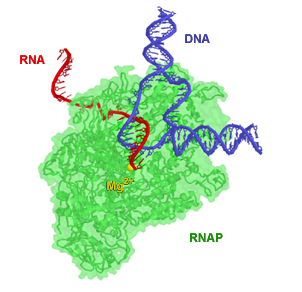
\includegraphics[width=\marginparwidth]{RNAP_TEC_small}
    Polymerases are a large, strongly conserved enzyme complexes consisting of
    multiple proteins}

Transcription of the mammalian genome is divided among multiple RNA polymerases
(Pol), each transcribing a non-overlapping set of genes. Messenger RNAs (mRNAs)
for protein-coding genes are synthesized by Pol~II, while the genes encoding
transfer RNAs (tRNAs) are transcribed by Pol~III. The direct interaction of
these transcripts produced by Pol~II and Pol~III is a vital step in the flow of
genetic information, in which the triplet codons in mRNAs are selectively
identified by their counterpart tRNA anticodons to direct protein synthesis. To
explore the largely unknown regulatory mechanisms active at this mRNA–tRNA
interface, we exploited the rapid and extensive changes in the transcriptome
occurring among different developmental stages of mammalian organogenesis
(Kyrmizi et al. 2006; Li et al. 2009; Kang et al. 2011; Lee et al. 2012;
Liscovitch and Chechik 2013; Sunkin et al. 2013).

Conceptually, one possible mechanism to control protein abundance in developing
tissues could be the deliberate mismatch of triplet codons in mRNAs and their
corresponding tRNA anticodon isoacceptors (Bra\-ck\-ley et al. 2011). In protozoa,
this strategy is used to modulate the rate of translation of specific subsets of
mRNAs containing a particular profile of codons (Horn 2008). Alternatively, if
the large-scale changes in protein-coding transcriptomes result in a stable
distribution of mRNA triplet codons, then deliberate changes in the population
of tRNA anticodons could be used to fine-tune protein translation.
Hypertranscription of tRNAs by Pol~III has been observed in cancers
\citep{Winter:2000, Pavon-Eternod:2009, Pavon-Eternod:2013}, with recent work
suggesting that differences in expression of specific tRNA genes may contribute
to tumourigenesis by favoring translation of cancer-promoting mRNAs driving
proliferation \citep{Pavon-Eternod:2009}. It is unknown whether normal
mammalian cells modulate tRNA gene expression to regulate information flow from
mRNAs to protein synthesis.
